\documentclass{article}

\usepackage{tikz}

\begin{document}

\begin{center}
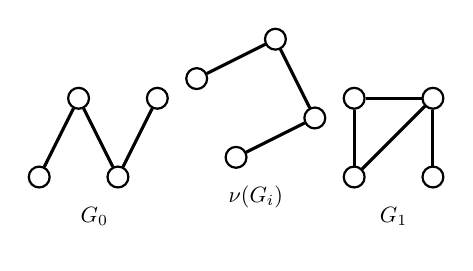
\begin{tikzpicture}[every node/.style={circle,thick,draw,scale=0.8}, line width=0.04cm]
    \node (A) at (0,-1.25) {};
    \node (B) at (1,-0.75) {};
    \node (C) at (-0.5,-0.25) {};
    \node (D) at (0.5,0.25) {};

    \draw (A) -- (B);
    \draw (B) -- (D);
    \draw (C) -- (D);

    \node[draw=none] (TEXT3) at (0.25,-1.75) {$\nu(G_i)$};

    \node (E) at (-1,-0.5) {};
    \node (F) at (-2,-0.5) {};
    \node (G) at (-2.5, -1.5) {};
    \node (H) at (-1.5, -1.5) {};

    \draw (G) -- (F);
    \draw (F) -- (H);
    \draw (H) -- (E);

    \node[draw=none] (TEXT) at (-1.8,-2) {$G_0$};

    \node (I) at (1.5, -0.5) {};
    \node (J) at (2.5,-0.5) {};
    \node (K) at (1.5,-1.5) {};
    \node (L) at (2.5,-1.5) {};

    \draw (I) -- (K);
    \draw (I) -- (J);
    \draw (K) -- (J);
    \draw (J) -- (L);

    \node[draw=none] (TEXT) at (2,-2) {$G_1$};
\end{tikzpicture}
\end{center}

\end{document}